%\lstset{
%basicstyle=\footnotesize\ttfamily, 
%otherkeywords={>>},
%keywordstyle=\ttfamily\bfseries,
%numbers=none,
%commentstyle=\color{blue}\sffamily\itshape,
%stringstyle=\color{black}\ttfamily 
%} 

In this chapter, we describe key \xten semantics and features to help readers 
unfamiliar with \xten to
have a better understanding of the \mixten compiler.   

\xten is an award winning open-source programming language being developed by
IBM Research. The goal of the \xten project is to provide a productive and
scalable programming model for the new-age high performance computing
architectures ranging from multi-core processors to clusters and
supercomputers~\cite{x10}. 

\xten, like Java, is a class-based, strongly-typed, garbage-collected and
object-oriented language. It uses Asynchronous Partitioned Global Address 
Space (APGAS)
model to support concurrency and distribution~\cite{specs}. The \xten compiler has a
\emph{native backend} that compiles \xten programs to C++ and a 
\emph{managed backend} that
compiles \xten programs to Java. 

In contrast to \xten, \matlab is a commercially-successful, proprietary
programming language that focuses on simplicity of implementing numerical
computation application~\cite{MatlabGrowth}. \matlab is a weakly-typed, dynamic language
with unconventional semantics and uses a JIT compiler backend.
It provides restricted support for high performance
computing via Mathworks' parallel computing toolbox~\cite{pct}. 

\section{Overview of \xten's key sequential features}

\xten's sequential core is a container-based object-oriented language that is 
very similar to that of Java or C++~\cite{specs}. A \xten program consists of a
collection of classes, structs or interfaces, which are the top-level compilation
units.
% Inheritance and subtyping are fairly conventional. 
\xten's sequential
constructs like \texttt{if}-\texttt{else} statements, \texttt{for} loops,
\texttt{while} loops, \texttt{switch} statements, and exception handling
constructs \texttt{throw} and \texttt{try}\ldots\texttt{catch} are also same 
as those in Java. 
\xten provides both, implicit coercions and explicit conversions on types, and 
both can
be defined on user-defined types. The \texttt{as} operator is used to perform
explicit type conversions; for example, \texttt{x as Long\{self != 0\}} converts
\texttt{x} to type \texttt{Long} and throws a runtime exception if its value is
zero. Multi-dimensional arrays in \xten are provided as user-defined abstractions on top of
\texttt{x10.lang.Rail}, an intrinsic one-dimensional array analogous to
one-dimensional arrays in languages like C or Java. Two families of
multi-dimensional array abstractions are provided: \emph{simple arrays}, which
provide
a restricted but efficient implementation, and \emph{region arrays} which
provide
a flexible and dynamic implementation but are not as efficient as \emph{simple
arrays}.
Listing \ref{lst:x10simple} shows a sequential 
\xten program that calculates the value of $\pi$
using the Monte Carlo method. It highlights important sequential and
object-oriented features of \xten detailed in the following subsections.

\begin{lstlisting}[caption={Sequential \xten program to calculate value of $\pi$
using Monte Carlo method},label={lst:x10simple},language=x10,numbers=none]
package examples;
import x10.util.Random;

public class SeqPi {
  public static def main(args:Rail[String]) {
    val N = Int.parse(args(0));
    var result:Double = 0;
    val rand = new Random();
    for(1..N) {
      val x = rand.nextDouble();
      val y = rand.nextDouble();
      if(x*x + y*y <= 1) result++;
    }
    val pi = 4*result/N;
    Console.OUT.println("The value of pi is " + pi);
  }
}

\end{lstlisting}

%\xten also provides very flexible
%arrays based on ideas in ZPL~\cite{}.  
\subsection{Object-oriented features}

A program consists of a collection of \emph{top-level units}, where a unit is
either a \emph{class}, a \emph{struct} or an \emph{interface}. A program can
contain multiple units, however only one unit can be made \texttt{public} and
its name must be same as that of the program file. Similar to Java, access to
these \emph{top-level units} is controlled by \emph{packages}. Below is a
description of the core object-oriented constructs in \xten: 

\begin{description}

\item[Class] A class is a basic bundle of data and code. It consists of zero or
more \emph{members} namely \emph{fields}, \emph{methods}, \emph{constructors},
and member classes and interfaces~\cite{x10intro}. It also specifies the name of its
\emph{superclass}, if any and of the interfaces it \emph{implements}.  

\item[Fields] A field is a data item that belongs to a class. It can be mutable
(specified by the keyword  \texttt{var}) or immutable (specified by the keyword
\texttt{val}). The type of a mutable field must be always be specified, however
the type of an immutable field may be omitted if it's declaration specifies an
\emph{initializer}. Fields are by default instance fields unless marked with the
\texttt{static} keyword. Instance fields are inherited by subclasses, however
subclasses can shadow inherited fields, in which case the value of the shadowed
field can be accessed by using the qualifier \texttt{super}.

%\item[Properties]

\item[Methods] A method is a named piece of code that takes zero or more
\emph{parameters} and returns zero or one value. The type of a method is
the type of the return value or \texttt{void} if it does not return a value.
If the return type of a method is not provided by the programmer, \xten infers
it as the least upper bound of the types of all expressions \texttt{e} in the
method where the body of the method contains the statement \texttt{return e}.
A method may have a type parameter that makes it \emph{type generic}. An
optional \emph{method guard} can be used to specify constraints. All methods in
a class must have a unique signature which consists of its name and types of its
arguments.     

Methods may be inherited. Methods defined in the superclass are available in the
subclasses, unless overridden by another method with same signature. Method
overloading allows programmer to define multiple methods with same name as long
as they have different signatures. Methods can be access-controlled to be
\texttt{private}, \texttt{protected} or \texttt{public}. \texttt{private}
methods can only be accessed by other methods in the same class.
\texttt{protected} methods can be accessed in the same class or its subclasses.
\texttt{public} methods can be accessed from any code. By default, all methods
are \emph{package protected} which means they can be accessed from any code in
the same package.

Methods with the same name as that of the containing class are called
constructors. They are used to instantiate a class. 

\item[Structs] A struct is just like a class, except that it does not support
inheritance and may not be recursive. This allows structs to be implemented as
\emph{header-less} objects, which means that unlike a class, a struct can be
represented by only as much memory as is necessary to represent its fields and
with its methods compiled to static methods. It does not contain a \emph{header}
that contains data to represent meta-information about the object. Current version
of \xten (version 2.4) does not support mutability and references to structs,
which means that there is no syntax to update the fields of a struct and structs
are always passed by value. 


\item[Function literals] \xten allows definition of functions via literals. A
function consists of a parameter list, followed optionally by a return type,
followed by \texttt{=>}, followed by the body (an expression). For example,
\texttt{(i:Int, j:Int) => (i<j ? foo(i) : foo(j))}, is a function that takes
parameters \texttt{i} and \texttt{j} and returns \texttt{foo(i)} if \texttt{i<j}
and \texttt{foo(j)} otherwise. A function can access immutable variables defined
outside the body.  
 
\end{description}

\subsection{Statements} \xten provides all the standard statements similar to
Java. Assignment, \texttt{if - else} and \texttt{while} loop statements are 
identical to those in Java.

\texttt{for} loops in \xten are more advanced and  apart 
from the standard C-like for loop, \xten
provides three different kinds of for loops:

\begin{description}

\item \textbf{\emph{enhanced} \texttt{for} loops} take an index 
specifier of the 
form \texttt{i in r}, where \texttt{r} is any
value that implements \texttt{x10.lang.Iterable[T]} for some type \texttt{T}.
Code listing \ref{lst:x10loop1} below shows 
an example of this kind of \texttt{for} loops:
\begin{lstlisting}[caption={Example of enhanced for loop},label={lst:x10loop1},language=x10,numbers=none]
def sum(a:Rail[Long]):Long{
	var result:Long = 0;
	for (i in a){
		result += i;
	}
	return result;
}
\end{lstlisting}

\item \textbf{\texttt{for} loops over \texttt{LongRange}} iterate over all
the values enumerated by a \texttt{\justify LongRange}. A \texttt{LongRange} is
instantiated by an expression like \texttt{e1..e2} and enumerates all the
integer values from \texttt{a} to \texttt{b} (inclusive) where \texttt{e1}
evaluates to \texttt{a} and \texttt{e2} evaluates to \texttt{b}. Listing
\ref{lst:x10loop2} below
shows an example of a \texttt{for} loop that uses \texttt{LongRange}:
\begin{lstlisting}[caption={Example of for loop over \texttt{LongRange}},label={lst:x10loop2},language=x10,numbers=none]
def sum(N:Long):Long{
	var result:Long = 0;
	for (i in 0..N){
		result += i;
	}
	return result;
}
\end{lstlisting}

\item \textbf{\texttt{for} loops over \texttt{Region}} allow to iterate over
multiple dimensions simultaneously. A \texttt{Region} is a data structure that
represents a set of \emph{points} in multiple dimensions. For instance, a
\texttt{Region} instantiated by the expression 
\texttt{\justify{Region.make(0..5,1..6)}}
creates a 2-dimensional region of \emph{points} \texttt{(x,y)} where \texttt{x}
ranges over \texttt{0..5} and \texttt{y} over \texttt{1..6}. The natural order
of iteration is lexicographic. Listing \ref{lst:x10loop3} below shows an example that calculates
the sum of coordinates of all points in a given rectangle:
\begin{lstlisting}[caption={Example of for loop over a 2-D \texttt{Region}},label={lst:x10loop3},language=x10,numbers=none]
def sum(M:Long, N:Long):Long{
	var result:Long = 0;
	val R:Region = x10.regionarray.Region.make(0..M,0..N);
	for ([x,y] in R){
		result += x+y;
	}
	return result;
}
\end{lstlisting}

%\item[Exception Handling]
 
\end{description}

\subsection{Arrays}

In order to understand the challenges of translating \matlab to \xten,
one must understand the different flavours and functionality of \xten
arrays.

At the lowest level of abstraction, \xten provides an intrinsic
one-dimensional fixed-size array  called \verb|Rail| which is indexed by
a \verb|Long| type value starting at \verb|0|.  This is the \xten
counterpart of built-in arrays in languages like C or Java.  In
addition, \xten provides two types of more sophisticated array
abstractions in packages, \verb|x10.array| and \verb|x10.regionarray|.

\begin{description}
\item[Rail-backed Simple arrays] are a high-performance abstraction for
multidimensional arrays in \xten that support only rectangular dense
arrays with zero-based indexing. Also, they support only up to three
dimensions (specified statically) and row-major ordering. These
restrictions allow effective optimizations on indexing operations on the
underlying \verb|Rail|.  Essentially, these multidimensional arrays map
to a \verb|Rail| of size equal to number of elements in the array, in a
row-major order.

\item[Region arrays] are much more flexible.  A \emph{region} is a
set of points of the same rank, where \texttt{Points} are the indexing
units for arrays. Points are represented as n-dimensional tuples of
integer values. The \verb|rank| of a point defines the dimensionality of
the array it indexes.  The rank of a region is the rank of its
underlying points.  Regions provide flexibility of shape and indexing.
\emph{Region arrays} are just a set of elements with each element mapped
to a unique point in the underlying region. The dynamicity of these
arrays come at the cost of performance.

\end{description}
Both types of arrays also support distribution across places.  A
\emph{place} is one of the central innovations in \xten, which permits
the programmer to deal with notions of locality.


\subsection{Types}

\xten is a statically type-checked language: Every variable and expression has 
a type that is known at compile-time and the compiler checks that the operations
performed on an expression are permitted by the type of that expression. 
The name \texttt{c} of a class or an interface is the most basic form of type in
\xten. There are no primitive types. 

\xten also allows \emph{type definitions}, that allow a simple name to be
supplied for a complicated type, and for type aliases to be defined. For
example, a type definition like \texttt{public static type bool(b:Boolean) =
Boolean\{self=b\}} allows the use of expression \texttt{bool(true)} as a
shorthand for type \texttt{Boolean\{self=true\}}.
%about type Any
%\xten also supports following forms of types:

\begin{description}

\item[Generic types] \xten's generic types allow classes and interfaces to be
declared parameterized by types. They allow the code for a class to be reused
unbounded number of times, for different concrete types, in a type-safe fashion. 
For instance, the listing \ref{lst:x10GenType} below shows a class 
\texttt{List[T]}, parameterized by
type \texttt{T}, that can be replaced by a concrete type like \texttt{Int} at
the time of instantiation (\texttt{var l:List[Int] = new List[Int](item)}).
\begin{lstlisting}[caption={},label={lst:x10GenType},language=x10,numbers=none]
class List[T]{
	var item:T;
	var tail:List[T]=null;
	def this(t:T){
		item=t;
	}
}
\end{lstlisting}
\xten types are available at runtime, unlike Java(which erases them). 
%Thus it is
%possible to overload types like \texttt{List[Int]} and \texttt{List[Float]}

\item[Constrained types] \xten allows the programmer to define \texttt{Boolean}
expressions (restricted) constraints on a type \texttt[T]. For example, a
variable of constrained type \texttt{Long\{self != 0\}} is of type \texttt{Long}
and has a constraint that it can hold a value only if it is not equal to
\texttt{0} and throws a runtime error if the constraint is not
satisfied. The permitted constraints include the predicates \texttt{==} and
\texttt{!=}. These
predicates may be applied to constraint terms. A constraint term is either a
final variable visible at the point of definition of the constraint, or the
special variable \texttt{self} or of the form \texttt{t.f} where \texttt{f} 
names a field, and \texttt{t} is
(recursively) a constraint term.  

\end{description} 

\section{Overview of \xten's concurrency features}

\xten is a high performance language that aims at providing productivity to the
programmer. To achieve that goal, it provides a simple yet powerful concurrency
model that provides four concurrency constructs that abstract away the low-level
details of parallel programming from the programmer, without compromising on
performance. \xten's concurrency model is based on the Asynchronous Partitioned
Global Address Space (APGAS) model~\cite{apgaspaper}. APGAS model has a concept
of global address space that allows a task in \xten to refer to any object
(local or remote). However, a task may operate only on an object that resides in
its partition of the address space (local memory). Each task, called an
\emph{activity}, runs asynchronously parallel to each other. A logical
processing unit in \xten is called a \emph{place}. Each \emph{place} can run
multiple \emph{activities}.    
%\subsection{The APGAS Model}
Following four types of concurrency constructs are provided by
\xten~\cite{x10intro}:

\subsection{Async} The fundamental concurrency construct in \xten is
\texttt{async}. The statement \texttt{async S} creates a new \emph{activity} to
execute \texttt{S} and returns immediately. The current activity and the
``forked" activity execute asynchronously parallel to each other and have access
to the same heap of objects as the current activity. They communicate with each
other by reading and writing shared variables. There is no restriction on
statement \texttt{S} and can contain any other constructs (including
\texttt{async}). \texttt{S} is also permitted to refer to any immutable variable
defined in lexically enclosing scope.

An activty is
the fundamental unit of execution in \xten. It may be thought of as a very
light-weight thread of execution. Each activity has its own control stack and
may invoke recursive method calls. Unlike Java threads, activities in \xten are
unnamed. Activities cannot be aborted or interrupted once they are in flight.
They must proceed to completion, either finishing correctly or by throwing an
exception. An activity created by \texttt{async S} is said to be \emph{locally
terminated} if \texttt{S} has terminated. It is said to be \emph{globally
terminated} if it has terminated locally and all activities spawned by it
recursively, have themselves globally terminated.
   
\subsection{Finish} Global termination of an activity can be converted to local
termination by using the \texttt{finish} construct. This is necessary when the
programmer needs to be sure that a statement \texttt{S} and all the activities
spawned transitively by \texttt{S} have terminated before execution of the next
statement begins. For instance in the listing \ref{lst:x10GenType} below, use of
\texttt{finish} ensures that the \texttt{Console.OUT.println("a(1) = " + a(1));}
statement is executed only after all the asynchronously executing operations
(\texttt{async a(i) *= 2;} have completed.

\begin{lstlisting}[caption={Example use of \texttt{finish} construct},label={lst:x10GenType},language=x10,numbers=none]
//...
//Create a Rail of size 10, with i'th element initialized to i 
val a:Rail[Long] = new Rail[Long](10,(i:Long)=>i);
finish for (i in 0..9){
//asynchronously double every value in the Rail
	async a(i) *= 2;
}
Console.OUT.println("a(1) = " + a(1));
//...
\end{lstlisting}

\subsection{Atomic} \texttt{atomic S} ensures that the statement (or set of
statements) \texttt{S} is
executed in a single step with respect to all other activities in the system.
When \texttt{S} is being executed in one activity all other activities
containing \texttt{s} are suspended. However, the \texttt{atomic} statement 
\texttt{S} must be 
\emph{sequential}, \emph{non-blocking} and \emph{local}. Consider the code
fragment in listing \ref{lst:x10Atomic}. It asynchronously adds \texttt{Long}
values to a linked-list \texttt{list} and simultaneously holds the size of the
list in a variable \texttt{size}. The use of \texttt{atomic} guarantees that no
other operation, in any activity, is executed in between (or simultaneously
with) these two operations, which is necessary to ensure correctness of the
program.

\begin{lstlisting}[caption={Example use of \texttt{atomic}
construct},label={lst:x10Atomic},language=x10,numbers=none]
//...
	finish for (i in 0..10){
		async add(i);
	}
//...
	def add(x:Long){
		atomic {
			this.list.add(x);
			this.size = this.size + 1;
		}
	}
//...
\end{lstlisting}

Note that, \texttt{atomic} is a syntactic sugar for the construct \texttt{when
(c) }. \texttt{when (c)} is the conditional atomic statement based on binary 
condition \texttt(c). Statement \texttt{when (c) S} executes statement
\texttt{S} atomically only when \texttt{c} evaluates to true; if it is false,
the execution blocks waiting for \texttt{c} to be true. Condition \texttt{c}
must be \emph{sequential}, \emph{non-blocking} and \emph{local}.

\subsection{At} A \emph{place} in \xten is the fundamental processing unit. It
is a collection of data and activities that operate on that data. A program is
run on a fixed number of places. The binding of places to hardware resources
(e.g. nodes in a cluster, accelerators) is provided externally by a
configuration file, independent of the program. 

\texttt{at} construct provides a place-shifting operation, that is used to force
execution of a statement or an expression at a particular place. An activity
executing \texttt{at (p) S} suspends execution at the current place; The object
graph $G$ at the current place whose roots are all the variables $V$ used in
\texttt{S}
is serialized, and transmitted to place \texttt{p}, deserialized 
(creating a graph $G'$
isomorphic to $G$), an environment is created with the variables $V$ bound to
the corresponding roots in $G'$, and \texttt{S} executed at \texttt{p} in this 
environment. On
local termination of \texttt{S}, computation 
resumes after \texttt{at (p) S} in the original
location. The object graph is not automatically transferred back to the
originating place when \texttt{S} terminates: any updates made to 
objects copied by an \texttt{at}
will not be reflected in the original object graph. 

\section{Overview of \xten's implementation and runtime}

In order to understand the compilation flow of the \mixten compiler and
enhancements made to the \xten compiler for efficient use of \xten as a target
language for \matlab, it is important to understand the design of the \xten
compiler and its runtime environment.  

\subsection{\xten implementation}
\xten is implemented as a source-to-source compiler that translates \xten
programs to either C++ or Java. This allows \xten to achieve critical
portability, performance and interoperability objectives. The generated C++ or
Java program is, in turn, compiled by the platform C++ compiler to an executable
or to class files by a Java compiler. The C++ backend is referred to as
\emph{Native \xten} and the Java backend is called \emph{Managed \xten}. 

The
source-to-source compilation approach provides 
three main advantages: (1) It makes \xten
available for a wide range of platforms; (2) It takes advantage of the
underlying classical and platform-specific optimizations in C++ or Java
compilers, while the \xten implementation includes only \xten specific
optimizations; and (3) It allows programmers to take advantage of the existing
C++ and Java libraries.

Figure \ref{fig:x10compiler} shows the overall architecture of the \xten
compiler~\cite{x10intro}.  
 
\begin{figure}[p]
    \centering
    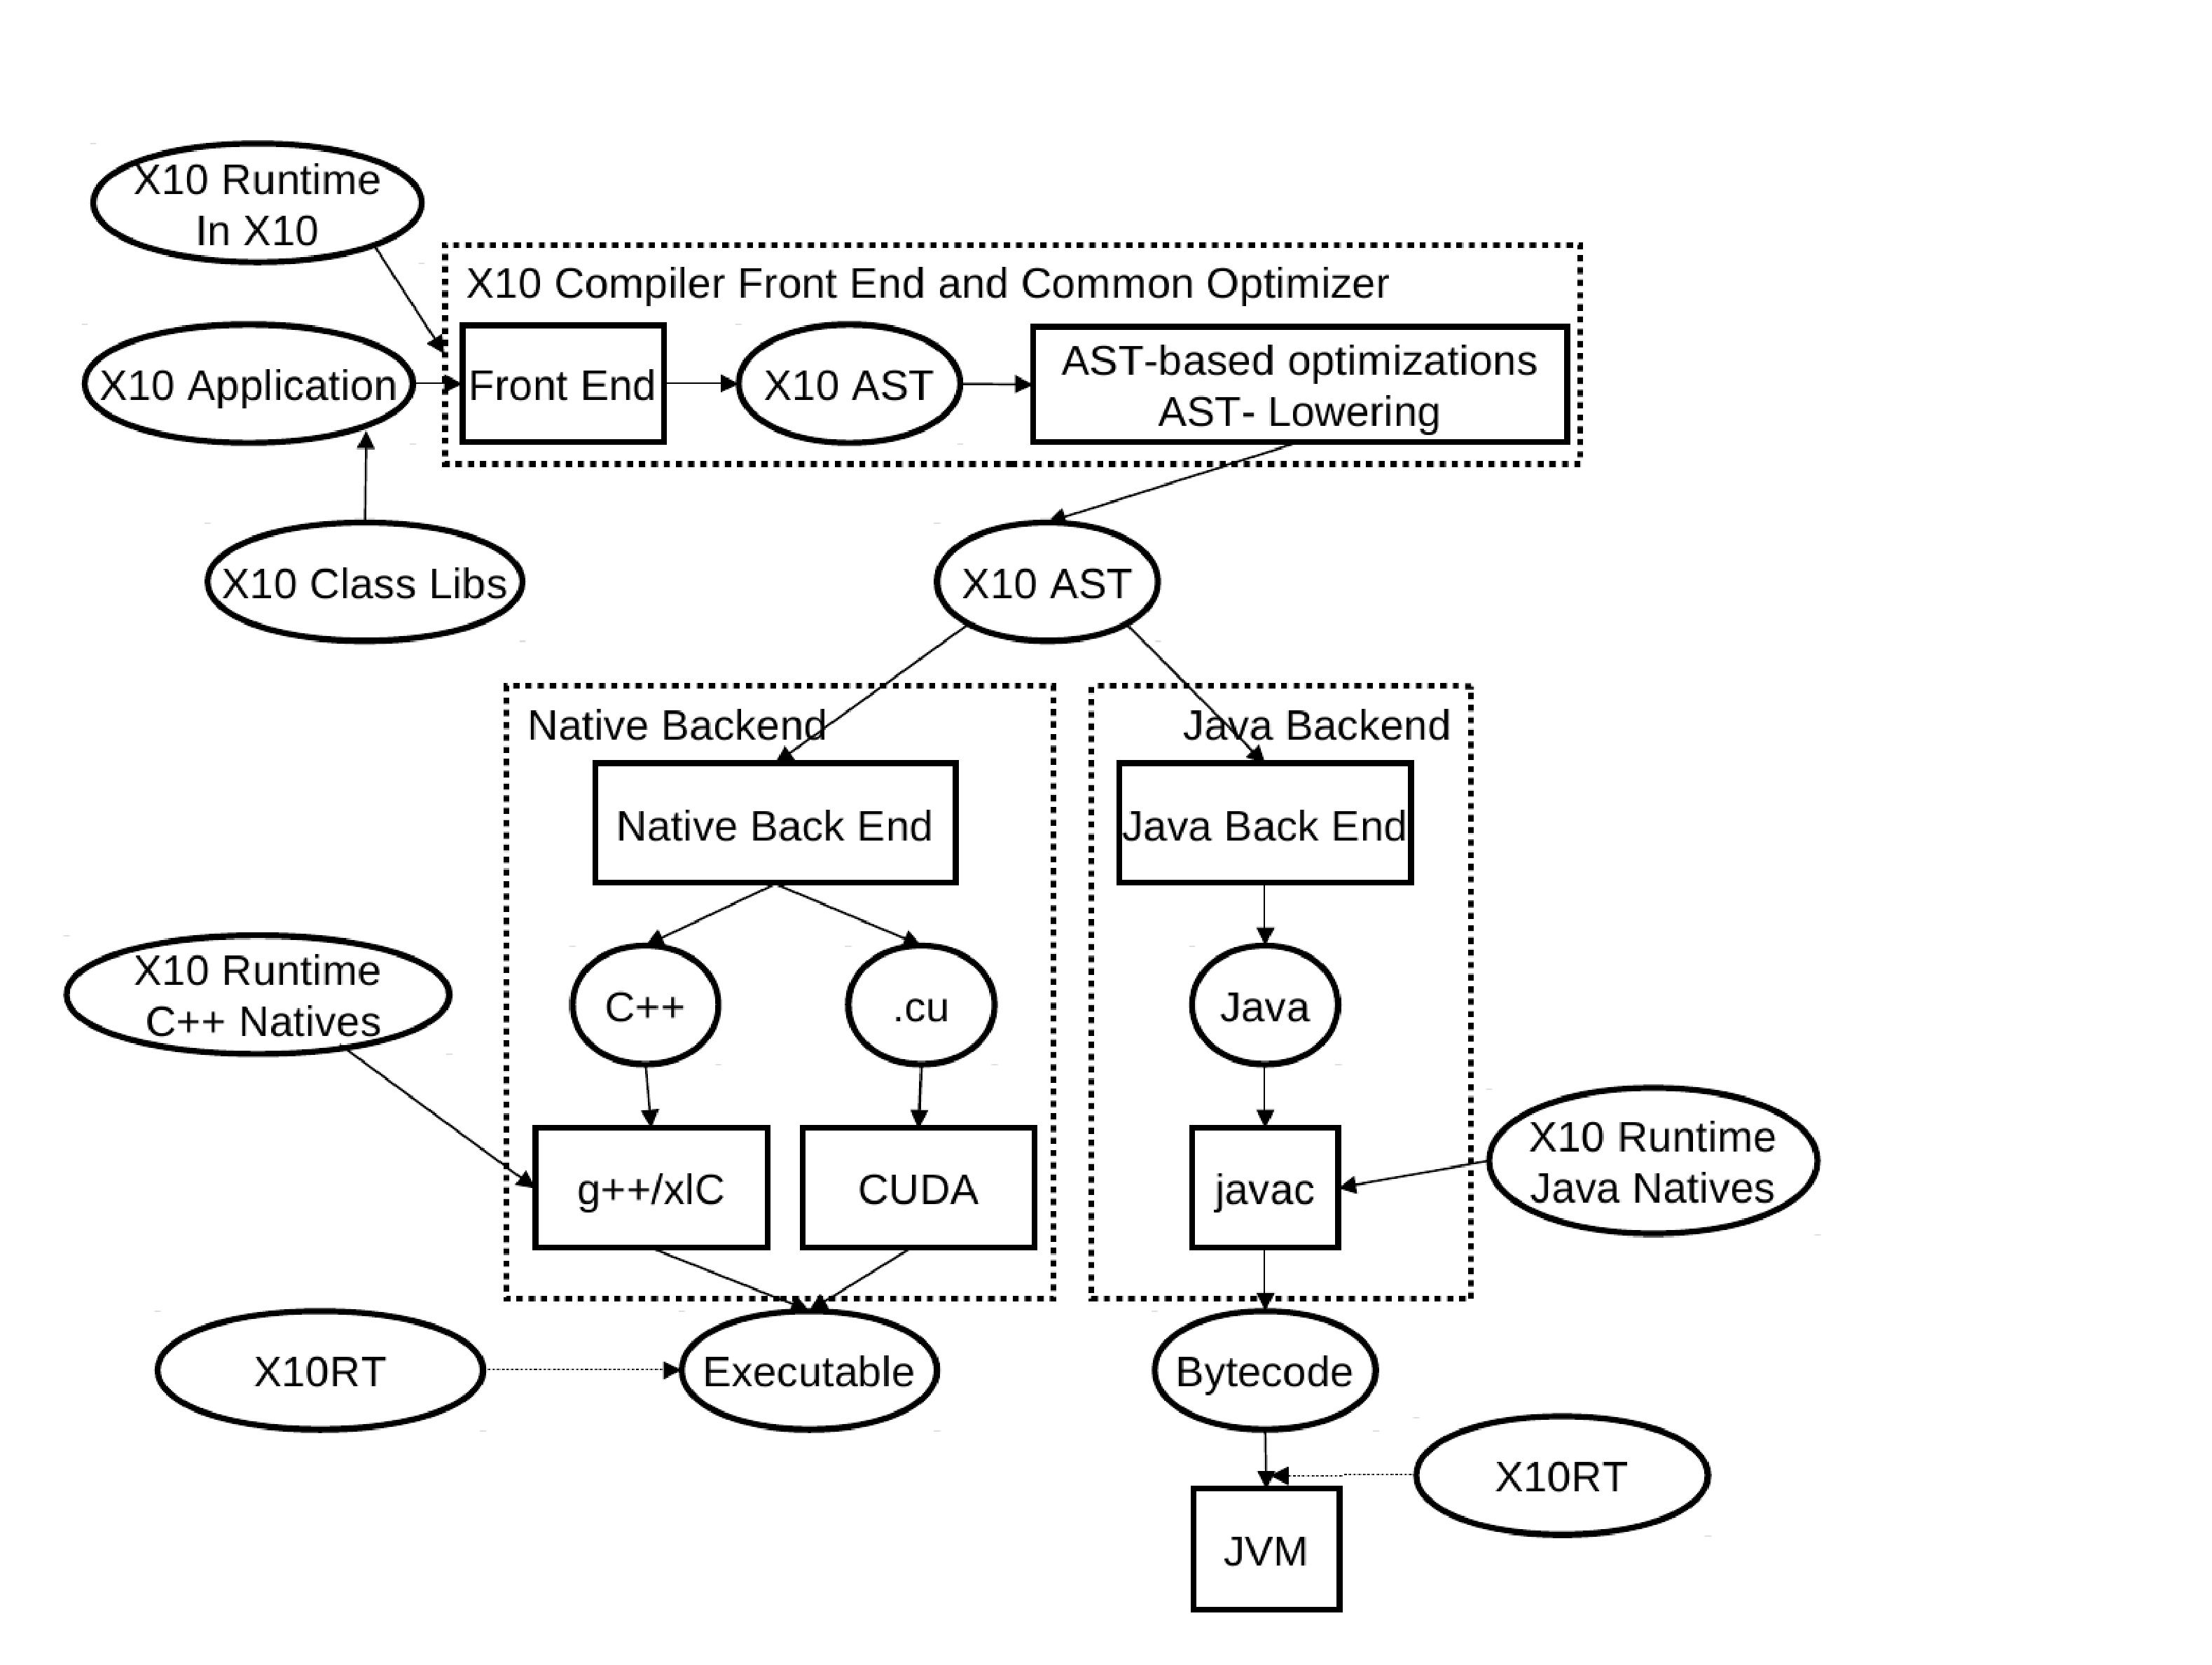
\includegraphics[width=0.8\textwidth]{Figures/x10compiler.eps}
    \caption{Architecture of the \xten compiler}
    \label{fig:x10compiler}
\end{figure}

\subsection{\xten runtime}
Figure \ref{fig:x10runtime} shows the major components of the \xten runtime and
their relative hierarchy~\cite{x10intro}. 

The runtime bridges the gap between 
application program and
the low-level network transport system and the operating system. X10RT, which is
the lowest layer of the \xten runtime, provides abstraction and unification of
the functionalities provided by various network layers. 

The \xten Language
Native Runtime provides implementation of the sequential core of the language.
It is implemented in C++ for native \xten and Java for Managed \xten. 

XRX Runtime, the \xten runtime in \xten is the core of the \xten runtime system.
It provides implementation for the primitive \xten constructs for concurrency
and distribution (\texttt{async}, \texttt{finish}, \texttt{atomic} and
\texttt{at}). It is primarily written in \xten over a set of low-level APIs that
provide a platform-independent view of processes, threads, synchronization
mechanisms and inter-process communication. 

At the top of the \xten runtime system, is a set of core
class libraries that provide fundamental data types, basic collections, and key
APIs for concurrency and distribution.   

\begin{figure}[p]
    \centering
    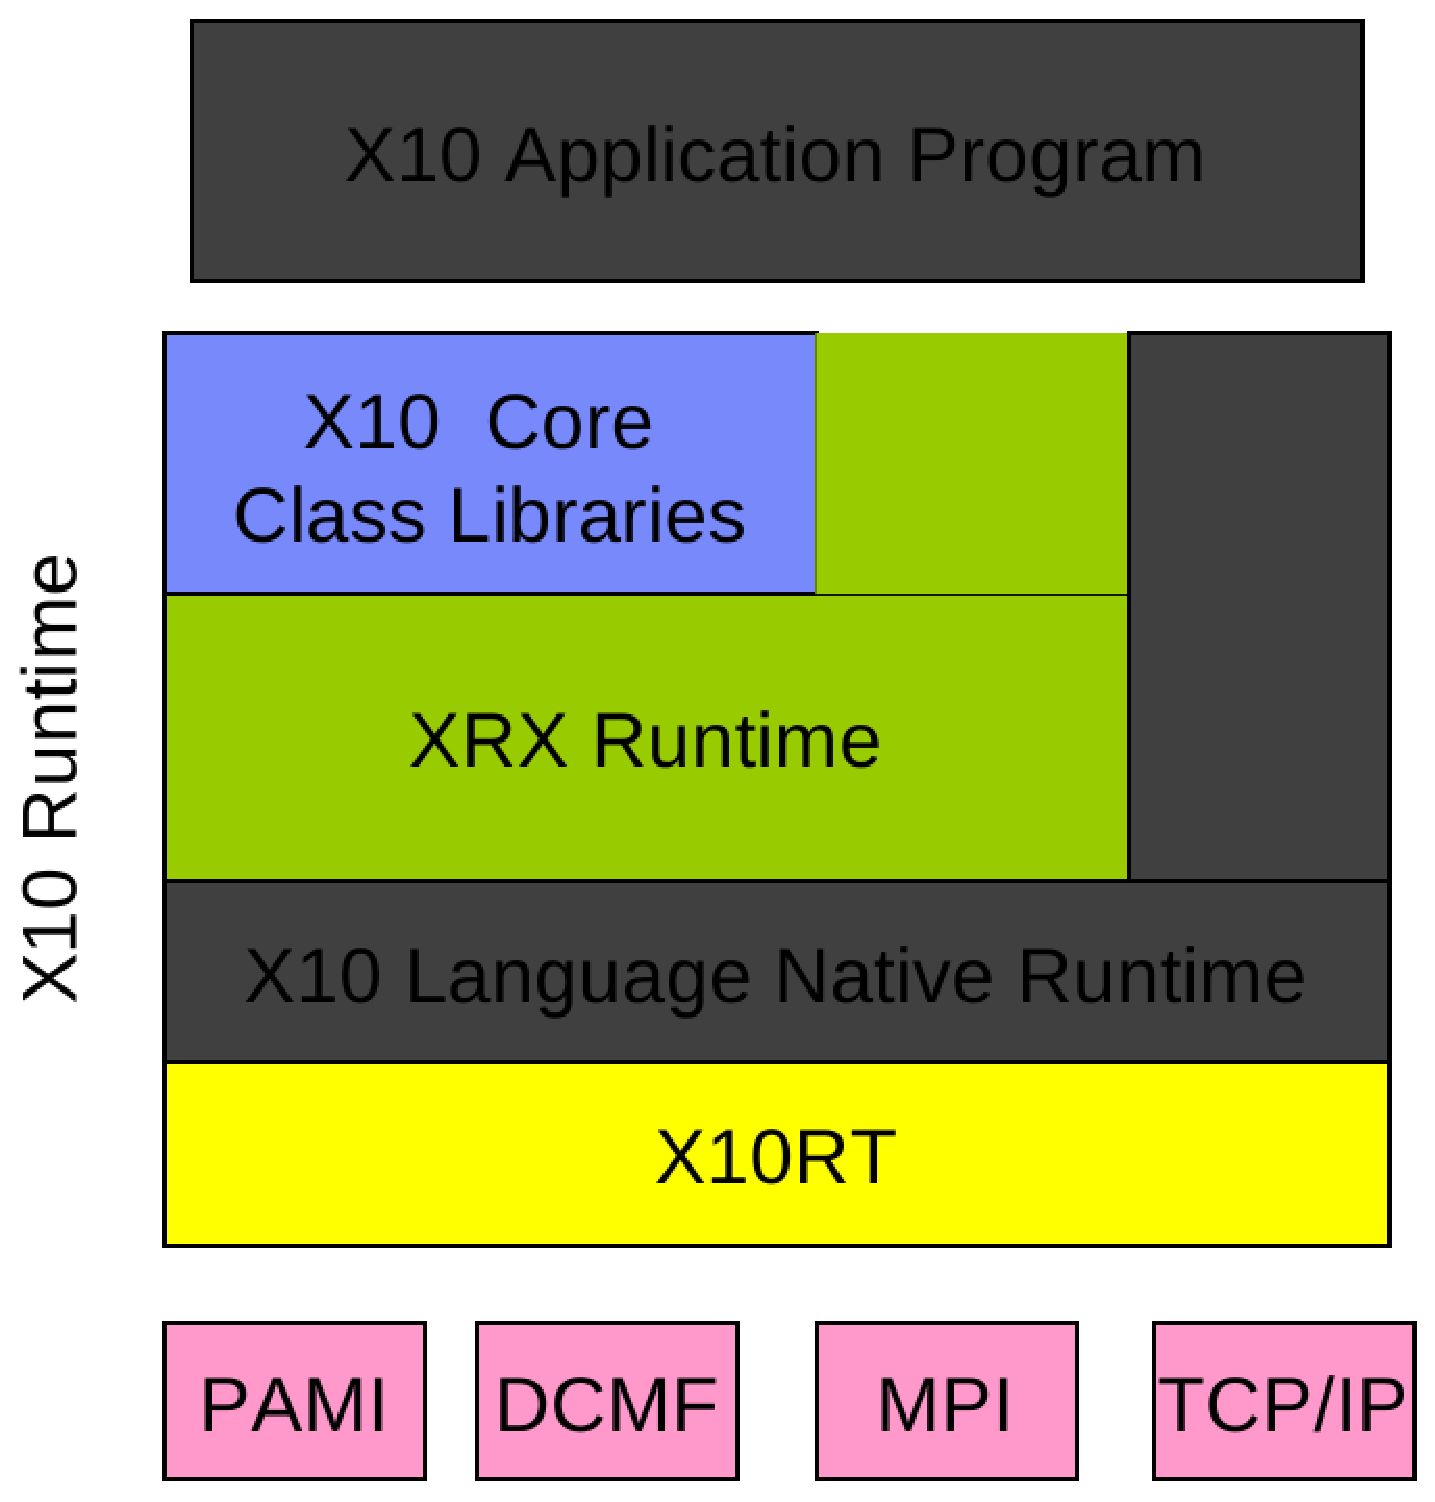
\includegraphics[width=0.8\textwidth]{Figures/x10runtime.eps}
    \caption{Architecture of the \xten runtime}
    \label{fig:x10runtime}
\end{figure}

\section{Summary}

In this chapter we have provided an overview of the key features of the \xten
programming language. In the following chapters, specially chapters
\chapref{chap:Codegen} and \chapref{chap:Arrays}, we will discuss some of the
features and constructs introduced here, in more depth. 

We will also discuss key constructs and features of the \matlab
programming language and contrast them with \xten, as we discuss \mixten's
compilation strategies in the following chapters. For readers who are completely
unfamiliar with \matlab or are interested in a quick overview, we suggest
reading chapter 2 of \cite{AntonThesis}.
   
